\apendice{Estudio experimental}

\section{Cuaderno de trabajo}

\subsection{Fase exploratoria inicial: predicción basada en datos reales del O2Ring}

El desarrollo del presente Trabajo de Fin de Grado comenzó con un enfoque centrado en la integración de variables fisiológicas reales, obtenidas mediante el dispositivo portátil \textbf{O2Ring} de Viatom. La idea inicial del proyecto era diseñar un sistema capaz de predecir alteraciones del sueño, no a partir de datos clínicos estáticos, sino utilizando señales biométricas registradas durante el descanso nocturno.

Para llevarlo a cabo, se combinó el uso del O2Ring con la administración del cuestionario de Pittsburgh (Pittsburgh Sleep Quality Index - PSQI) en formato digital \footnote{\href{https://forms.gle/3AVK69kD5NRKk4AP9}{Enlace al Test de Pittsburgh generado mediante Google Forms.}}. Este cuestionario permite evaluar la calidad subjetiva del sueño del paciente y estaba destinado a complementar la información objetiva recogida por el wearable.

\begin{figure}[H]
    \centering
    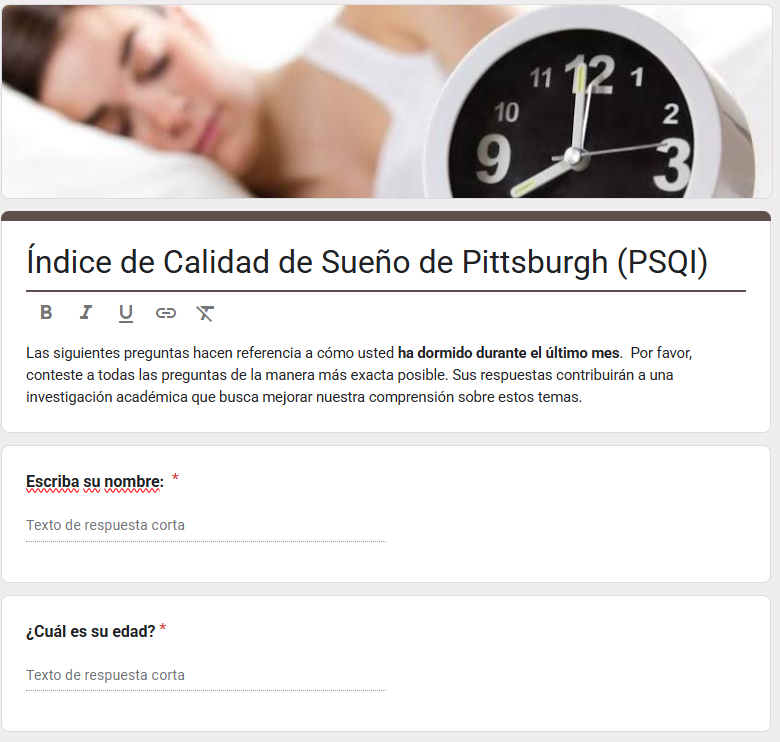
\includegraphics[width=0.5\linewidth]{img/pittsburgh.png}
    \caption{Test de Pittsburgh realizado mediante Google Forms.}
    \label{fig:pittsburgh}
\end{figure}

En esta primera fase, participaron varios voluntarios que utilizaron el anillo durante una o dos noches en su domicilio, con el objetivo de obtener mediciones completas y representativas. El O2Ring registró variables como la saturación de oxígeno (SpO$_2$), la frecuencia cardíaca, el número de eventos de desaturación y el índice de desaturación de oxígeno. De forma paralela, los participantes rellenaron el PSQI, cuyos resultados fueron codificados en una escala numérica. 

La idea era construir un modelo de predicción que, a partir de estas variables fisiológicas, clasificara la calidad del sueño en tres clases: buena, regular o mala. Para ello, se integraron todos los datos en cuadernos Jupyter y se procesaron con librerías como Pandas, Scikit-learn, Matplotlib y Seaborn. También se experimentó con técnicas de aumentación de datos, como la generación de ejemplos sintéticos mediante redes generativas adversarias (GANs) y autoencoders variacionales (VAEs).

Sin embargo, esta línea de trabajo resultó poco viable debido a la escasa disponibilidad de registros reales. Las dificultades para reunir una muestra lo suficientemente grande y balanceada, junto con la variabilidad individual de las señales, imposibilitaron el entrenamiento de un modelo robusto con garantías mínimas de generalización. La opción de aumentar los datos sintéticamente no solucionó del todo este problema, ya que los patrones de sueño requieren cierta estabilidad y validez clínica.

A pesar de que esta fase no pudo completarse con un modelo funcional, resultó verdaderamente útil para la comprensión de las variables fisiológicas recogidas, así como el verdadero proceso de adquisición de datos reales y su preprocesamiento.
 
\begin{figure}[H]
\centering

\includegraphics[width=0.4\textwidth]{o2ring.jpg}
\caption{Dispositivo O2Ring (Viatom) utilizado en la fase exploratoria inicial del proyecto. Fuente: \cite{o2ring_ifdesign}.}
\label{fig:o2ring}
\end{figure}

\subsection{Cambio de enfoque: utilización de datos clínicos estructurados}
Tras analizar los límites del enfoque inicial, y en coordinación con el tutor, se decidió reformular el enfoque del proyecto para adaptarlo a las limitaciones reales del entorno y los datos disponibles. El nuevo objetivo consistía en desarrollar una aplicación web predictiva utilizando un conjunto de datos clínico abierto y tabular, que facilitara el uso de algoritmos de aprendizaje automático con mayor volumen de registros y variables estructuradas.

El nuevo dataset, obtenido de la plataforma Kaggle\footnote{Dataset utilizado para el proyecto: \cite{alnour2024kaggle}.}, incluía información clínica, demográfica y de estilo de vida de más de 370 personas, con variables como edad, ocupación, duración del sueño, presión arterial, frecuencia cardíaca, pasos diarios y calidad del sueño percibida. Este conjunto permitía abordar un problema de clasificación multiclase con tres categorías: insomnio, apnea del sueño y sin trastorno.

A partir de este nuevo enfoque, se llevaron a cabo distintas fases: la exploración del conjunto de datos, su preprocesamiento, el entrenamiento y evaluación de distintos modelos de clasificación, la calibración de probabilidades, la explicación de resultados mediante SHAP y el desarrollo de la aplicación web.

\subsection{Configuración y parametrización de las técnicas}

Durante la fase experimental se evaluaron distintos algoritmos de clasificación con el objetivo de seleccionar el modelo más adecuado para la predicción multiclase del tipo de trastorno del sueño. Para ello, se utilizaron técnicas de validación cruzada, balanceo de clases y ajuste de hiperparámetros mediante \texttt{GridSearchCV} o \texttt{RandomizedSearchCV}, según el modelo.

\subsubsection{Regresión logística}

Se utilizó el modelo \texttt{LogisticRegression} de \texttt{scikit-learn}, con un número máximo de iteraciones ajustado a 5000 para asegurar la convergencia. La búsqueda de hiperparámetros se llevó a cabo mediante \texttt{GridSearchCV}, ya que se trata de un modelo con pocos parámetros, lo que permite evaluar exhaustivamente todas las combinaciones.

\begin{itemize}
    \item \textbf{penalty}: tipo de regularización aplicada.
    \begin{itemize}
        \item \texttt{l1}: penaliza la suma de los valores absolutos de los coeficientes. Favorece modelos más simples eliminando algunos coeficientes (lleva a cero).
        \item \texttt{l2}: penaliza la suma de los cuadrados de los coeficientes. Reduce su magnitud sin eliminarlos.
    \end{itemize}
    \item \textbf{C}: inverso de la fuerza de regularización. Valores pequeños implican regularización fuerte (modelo más simple), valores grandes permiten más flexibilidad.
    \item \textbf{solver}: algoritmo de optimización.
    \begin{itemize}
        \item \texttt{liblinear}: eficiente en conjuntos de datos pequeños, compatible con \texttt{l1} y \texttt{l2}.
        \item \texttt{saga}: escalable y compatible con regularización l1.
    \end{itemize}
\end{itemize}

La validación cruzada se realizó con \texttt{cv=5} usando precisión como métrica. La mejor combinación fue \texttt{penalty='l2'}, \texttt{C=10} y \texttt{solver='liblinear'}.

\subsubsection{Árboles de decisión}

El modelo \texttt{DecisionTreeClassifier} se entrenó ajustando sus hiperparámetros con \texttt{GridSearchCV}. Este tipo de modelo tiene como ventaja su capacidad de interpretar fácilmente las decisiones, aunque tiende a sobreajustarse si no se limita su complejidad.

\begin{itemize}
    \item \textbf{max\_depth}: controla la profundidad máxima del árbol. Profundidades mayores permiten mayor capacidad de aprendizaje, pero también riesgo de sobreajuste.
    \item \textbf{min\_samples\_split}: número mínimo de muestras necesarias para dividir un nodo. Valores más altos impiden que el árbol crezca innecesariamente.
    \item \textbf{min\_samples\_leaf}: número mínimo de muestras necesarias en una hoja del árbol. Ayuda a mantener ramas robustas.
    \item \textbf{criterion}: función usada para medir la calidad de una división.
    \begin{itemize}
        \item \texttt{gini}: mide la impureza de Gini.
        \item \texttt{entropy}: basada en la entropía de la teoría de la información.
    \end{itemize}
\end{itemize}

Se probaron varias combinaciones con \texttt{cv=5}. La mejor configuración utilizó \texttt{criterion= 'gini'} y sin límite de profundidad.

\subsubsection{Máquinas de vectores soporte (SVM)}

Se empleó la clase \texttt{SVC} y se utilizó \texttt{RandomizedSearchCV} para reducir el coste computacional, dado el número de combinaciones posibles entre hiperparámetros.

\begin{itemize}
    \item \textbf{C}: penalización por error. Valores altos intentan clasificar todos los datos correctamente, lo que puede derivar en sobreajuste.
    \item \textbf{kernel}: función que transforma los datos en un espacio de mayor dimensión.
    \begin{itemize}
        \item \texttt{linear}: separador lineal.
        \item \texttt{rbf}: radial basis function, muy flexible.
        \item \texttt{poly}: permite fronteras polinómicas.
        \item \texttt{sigmoid}: imita comportamiento de redes neuronales.
    \end{itemize}
    \item \textbf{gamma}: controla la influencia de cada punto. 
    \begin{itemize}
        \item \texttt{scale}: valor adaptado automáticamente.
        \item \texttt{auto}: inverso del número de características.
    \end{itemize}
\end{itemize}

Se probaron 20 combinaciones con \texttt{cv=5}. El mejor modelo tuvo \texttt{kernel='poly'}, \texttt{gamma='scale'} y \texttt{C=10}.

\subsubsection{Perceptrón multicapa (MLP)}

Se utilizó \texttt{MLPClassifier}, un modelo de red neuronal que permite aprender patrones no lineales complejos. Se aplicó \texttt{RandomizedSearchCV}, ya que el ajuste fino de parámetros puede ser costoso computacionalmente.

\begin{itemize}
    \item \textbf{hidden\_layer\_sizes}: número y tamaño de las capas ocultas. Se probaron estructuras como (50,), (100,) y (50,50).
    \item \textbf{activation}: función de activación en cada neurona.
    \begin{itemize}
        \item \texttt{relu}: rectificador lineal unipolar.
        \item \texttt{tanh}: función hiperbólica, útil en redes profundas.
    \end{itemize}
    \item \textbf{solver}: algoritmo de optimización.
    \begin{itemize}
        \item \texttt{adam}: adaptativo, robusto para muchos problemas.
        \item \texttt{sgd}: descenso por gradiente estocástico.
    \end{itemize}
    \item \textbf{alpha}: regularización L2 para evitar sobreajuste.
    \item \textbf{learning\_rate}: tipo de estrategia para modificar la tasa de aprendizaje durante el entrenamiento.
\end{itemize}

El mejor modelo utilizó \texttt{activation='tanh'}, \texttt{alpha=0.01}, \texttt{solver='adam'} y estructura \texttt{(50,)}.

\subsubsection{Random Forest}

Finalmente, se utilizó \texttt{RandomForestClassifier}, un modelo de conjunto basado en árboles de decisión. Se aplicó \texttt{RandomizedSearchCV} para evaluar combinaciones de hiperparámetros de forma eficiente.

\begin{itemize}
    \item \textbf{n\_estimators}: número de árboles en el bosque.  Más árboles generalmente mejoran el rendimiento, pero aumentan el tiempo de entrenamiento.
    \item \textbf{max\_depth}: profundidad máxima de cada árbol.
    \item \textbf{min\_samples\_split}: número mínimo de muestras necesarias para dividir un nodo.
    \item \textbf{min\_samples\_leaf}: número mínimo de muestras por hoja.
    \item \textbf{bootstrap}: si se realiza muestreo con reemplazo al construir los árboles.
\end{itemize}

Se probaron 20 combinaciones con validación cruzada. El modelo final utilizó \texttt{n\_estimators=200}, \texttt{max\_depth=None} y \texttt{bootstrap=True}, mostrando gran robustez, precisión y compatibilidad con técnicas de interpretación como SHAP.


\subsubsection{Resumen y elección del modelo final}

Tras comparar el rendimiento de los modelos evaluados, el clasificador \texttt{Random Forest} fue seleccionado como el modelo final a integrar en el sistema. Esta decisión se basó en su:

\begin{itemize}
    \item Alto rendimiento general en precisión, F1-score y estabilidad.
    \item Capacidad para manejar conjuntos de datos con variables categóricas y numéricas sin necesidad de transformaciones complejas.
    \item Robustez frente al sobreajuste, gracias a la agregación de múltiples árboles.
    \item Compatibilidad con técnicas de interpretabilidad, como SHAP, que permiten explicar la predicción individual y global de manera visual y comprensible.
\end{itemize}

En el siguiente apartado (\nameref{sec:resultados}), se presentan las métricas obtenidas en la validación cruzada y los resultados más representativos del modelo entrenado y calibrado.

\subsection{Desarrollo de la aplicación y síntesis de resultados}

Como parte final del desarrollo, se diseñó e implementó una aplicación web interactiva mediante \texttt{Streamlit}. Esta app permite introducir manualmente variables clínicas y de estilo de vida, ejecutar el modelo predictivo, visualizar una explicación local de la predicción (mediante SHAP) y generar un informe en formato PDF con los resultados.

Durante esta fase, se abordaron cuestiones como la validación de entrada, el formateo automático del informe, la exportación de gráficos y la integración con el modelo calibrado previamente entrenado y almacenado con \texttt{joblib}.

La app fue probada con diversos perfiles clínicos simulados, y se validó su funcionamiento en sesiones reales. Además, se realizaron ajustes en el diseño visual y en la generación de resultados con fines interpretativos y de presentación clínica.

En cuanto a los resultados, el modelo seleccionado (Random Forest calibrado) obtuvo una precisión media del 84\% en validación cruzada. La clase ‘None’ fue la más fácilmente reconocible, mientras que la clase ‘Sleep Apnea’ fue la más proclive a falsos positivos. Estos patrones se confirmaron también en la validación externa con datos reales del O2Ring, lo que destaca tanto las capacidades actuales del sistema como las áreas de mejora futura.


\section{Detalle de resultados}
\label{sec:resultados}

El modelo final, Random Forest calibrado, fue evaluado sobre un conjunto de test independiente compuesto por 75 muestras. Las métricas por clase se muestran a continuación:

\begin{table}[H]
\centering
\begin{tabular}{|l|c|c|c|c|}
\hline
\textbf{Clase} & \textbf{Precisión} & \textbf{Recall} & \textbf{F1-score} & \textbf{Soporte} \\
\hline
Insomnia      & 0.93 & 0.93 & 0.93 & 15 \\
None          & 1.00 & 1.00 & 1.00 & 44 \\
Sleep Apnea   & 0.94 & 0.94 & 0.94 & 16 \\
\hline
\textbf{Media macro} & 0.96 & 0.96 & 0.96 & 75 \\
\textbf{Media ponderada} & 0.97 & 0.97 & 0.97 & 75 \\
\hline
\end{tabular}
\caption{Métricas del modelo Random Forest calibrado sobre el conjunto de test.}
\end{table}

\subsection{Evaluación comparativa: impacto de la variable Occupation}

Con el objetivo de analizar el impacto de la variable \texttt{Occupation} en el rendimiento clínico del modelo, se desarrolló una versión alternativa del sistema predictivo excluyendo dicha variable. Esta decisión se fundamenta en la posibilidad de que ciertas ocupaciones actúen como proxies de factores estructurales no controlados, como el estilo de vida o el nivel socioeconómico, generando sesgos en el diagnóstico automático.

Para comparar el comportamiento de ambas versiones, se evaluaron tres perfiles clínicos reales (Pacientes A, B y C) con ambos modelos, registrando las clases predichas y sus probabilidades asociadas. Se mantuvieron fijos los parámetros clínicos extraídos de los informes del O2Ring (edad, sexo, IMC, FC) y se ajustaron únicamente las variables no presentes en dichos informes (como pasos diarios, nivel de estrés o calidad del sueño) para evitar contradicciones y mejorar la coherencia diagnóstica esperada.

\begin{table}[H]
\centering
\begin{tabular}{|c|c|c|c|c|}
\hline
\textbf{Paciente} & \textbf{Diagnóstico esperado} & \textbf{Con Occupation} & \textbf{Sin Occupation} \\
\hline
A – Apnea & Apnea moderada-grave & Apnea (70.0\%) & Insomnio (59.0\%) \\
B – Sano & Sin trastornos & Apnea (59.0\%) & None (98.0\%) \\
C – Insomnio & Insomnio leve & Apnea (58.0\%) & None (79.0\%) \\
\hline
\end{tabular}
\caption{Comparativa entre versiones del modelo para los tres perfiles clínicos reales.}
\end{table}

Los resultados muestran un patrón claro: el modelo entrenado con la variable \texttt{Occupation} tiende a sobrediagnosticar apnea del sueño, clasificando todos los perfiles como tal incluso cuando no existe evidencia clínica suficiente (como en los pacientes B y C).

Por el contrario, el modelo sin \texttt{Occupation} mostró un comportamiento más prudente y alineado con los perfiles clínicos reales, especialmente en el caso del paciente sano (B), al que clasificó correctamente con una alta probabilidad. Si bien aún existen errores en el diagnóstico de insomnio, la eliminación de \texttt{Occupation} permitió reducir el sesgo observado hacia la clase de apnea.

Este experimento refuerza la necesidad de evaluar cuidadosamente el impacto de variables socioeconómicas en sistemas de ayuda al diagnóstico. En consecuencia, se optó por incluir \texttt{Occupation} en la versión final del modelo desplegado en la aplicación, priorizando la robustez y la interpretabilidad.


\section{Validación externa con datos reales del O2Ring}

Con el fin de evaluar el comportamiento del modelo ante datos reales, se utilizó información fisiológica de tres pacientes reales monitorizados mediante el dispositivo O2Ring. Los casos fueron seleccionados para representar tres perfiles clínicos distintos: apnea del sueño, sujeto sano e insomnio leve.

\subsection{Paciente A – Apnea del sueño}
\begin{itemize}
    \item Edad: 57 años, IMC: 31.8
    \item SpO$_2$ media: 89\%, mínima: 70\%
    \item ODI 3\%: 43.3/h, FC media: 61 bpm
    \item Predicción del modelo: \texttt{Sleep Apnea} (70.4\%) 
\end{itemize}

\subsection{Paciente B – Perfil sano}
\begin{itemize}
    \item Edad: 31 años, IMC: 25.1
    \item SpO$_2$ media: 97\%, mínima: 95\%
    \item ODI 3\%: 0.0/h, FC media: 58 bpm
    \item Predicción del modelo: \texttt{Sleep Apnea} (59.3\%) 
\end{itemize}

\subsection{Paciente C – Insomnio leve}
\begin{itemize}
    \item Edad: 55 años, IMC: 25.4
    \item Duración del sueño: 7.0h, calidad baja, estrés muy alto
    \item SpO$_2$ media: 95\%, ODI 3\%: 4.1/h
    \item FC media: 48 bpm
    \item Predicción del modelo: \texttt{Sleep Apnea} (72.7\%) 
\end{itemize}

\begin{table}[H]
\centering
\begin{tabular}{|c|c|c|c|c|}
\hline
\textbf{Paciente} & \textbf{Diagnóstico esperado} & \textbf{Predicción} & \textbf{Probabilidad} & \textbf{¿Acertó?} \\
\hline
A & Apnea del sueño & Sleep Apnea & 70.4\% & Sí \\
B & Sin trastornos & Sleep Apnea & 59.3\% & No \\
C & Insomnio leve & Sleep Apnea & 72.7\% & No \\
\hline
\end{tabular}
\caption{Resumen de resultados en la validación externa con datos reales.}
\end{table}


\subsection{Discusión}

Aunque el modelo mostró un rendimiento sólido en validación cruzada, la validación externa con datos fisiológicos reales puso de manifiesto varias limitaciones importantes. En concreto, dos de los tres pacientes fueron clasificados incorrectamente como casos de apnea del sueño, a pesar de presentar valores normales de saturación de oxígeno (SpO$_2$), frecuencia cardíaca y un índice ODI bajo o compatible con insomnio leve.

Este comportamiento sugiere una tendencia del sistema a sobrediagnosticar apnea, probablemente como resultado del desbalance en el dataset original o del peso excesivo asignado a variables indirectas como la ocupación. La comparación con una versión alternativa del modelo que excluía la variable \texttt{Occupation} confirmó esta hipótesis: dicho modelo mostró un comportamiento más prudente y, en varios casos, ofreció predicciones más acordes con el perfil clínico real.

No obstante, se optó por mantener el modelo con \texttt{Occupation} en la versión final de la aplicación por motivos de estabilidad técnica, calibración ya validada, y compatibilidad con el sistema de visualización e interpretación integrado. Esta decisión no implica ignorar sus limitaciones, sino gestionarlas de forma responsable: la aplicación incorpora un informe clínico descargable, un sistema de interpretabilidad mediante SHAP y una advertencia explícita sobre la naturaleza orientativa del sistema.

En conjunto, la validación externa desempeñó un papel clave al evidenciar las debilidades reales del modelo y al permitir evaluar su comportamiento en un contexto clínico simulado. Esta experiencia pone de manifiesto la necesidad de integrar señales fisiológicas en futuras versiones del sistema (como SpO$_2$ u ODI en tiempo real), así como de ampliar y diversificar el conjunto de entrenamiento con perfiles reales y clínicamente etiquetados. Solo mediante ese enfoque podrá garantizarse que este tipo de herramientas ofrezcan una ayuda diagnóstica fiable y sin sesgos.



\subsection{Informe clínico del dispositivo O2Ring}

Los datos fisiológicos utilizados en la validación externa fueron extraídos directamente de los informes generados por el dispositivo \textbf{O2Ring} tras su uso durante una noche completa de sueño. Estos informes, generados en formato PDF mediante el software oficial O$_2$ Insight Pro, recogen métricas como la saturación de oxígeno (SpO$_2$), los eventos de desaturación (ODI 3\% y 4\%), la frecuencia cardíaca (FC) y el tiempo acumulado con valores críticos de oxígeno.

A continuación, se presenta como ejemplo el informe correspondiente al \textbf{Paciente A}, en el que se puede observar una puntuación O2 reducida, una SpO$_2$ media de 89\%, con desaturaciones severas frecuentes y un índice ODI 3\% de 43.3 eventos por hora, lo que es clínicamente compatible con un caso de apnea del sueño moderada-grave.

\begin{table}[H]
    \centering
    \begin{tabular}{|l|c|}
    \hline
    \textbf{Parámetro} & \textbf{Valor} \\
    \hline
    Duración total & 5h 53m \\
    SpO$_2$ media & 89\% \\
    SpO$_2$ mínima & 70\% \\
    ODI 3\% & 43.3 eventos/hora \\
    Frecuencia cardíaca media & 61 bpm \\
    \hline
    \end{tabular}
    \caption{Resumen de parámetros extraídos del informe del Paciente A.}
\end{table}

Además de los valores numéricos, el informe incluye gráficas de evolución temporal de SpO$_2$, frecuencia cardíaca y movimiento. A nivel visual, se aprecia un patrón repetitivo de desaturaciones rápidas seguido de recuperaciones bruscas, visibles especialmente entre las 02:30 y las 05:30. Durante este intervalo, la SpO$_2$ cae de forma reiterada por debajo del umbral clínico del 90\%, alcanzando incluso valores mínimos cercanos al 70\%.

También se observan variaciones sincronizadas en la frecuencia cardíaca, que muestra picos coincidentes con algunos eventos de desaturación, así como incrementos en el movimiento. Esta combinación de oscilaciones de SpO$_2$, activación autonómica y actividad motora nocturna es característica de pacientes con apnea obstructiva del sueño y refuerza la validez clínica del informe.


\begin{figure}[H]
    \centering
    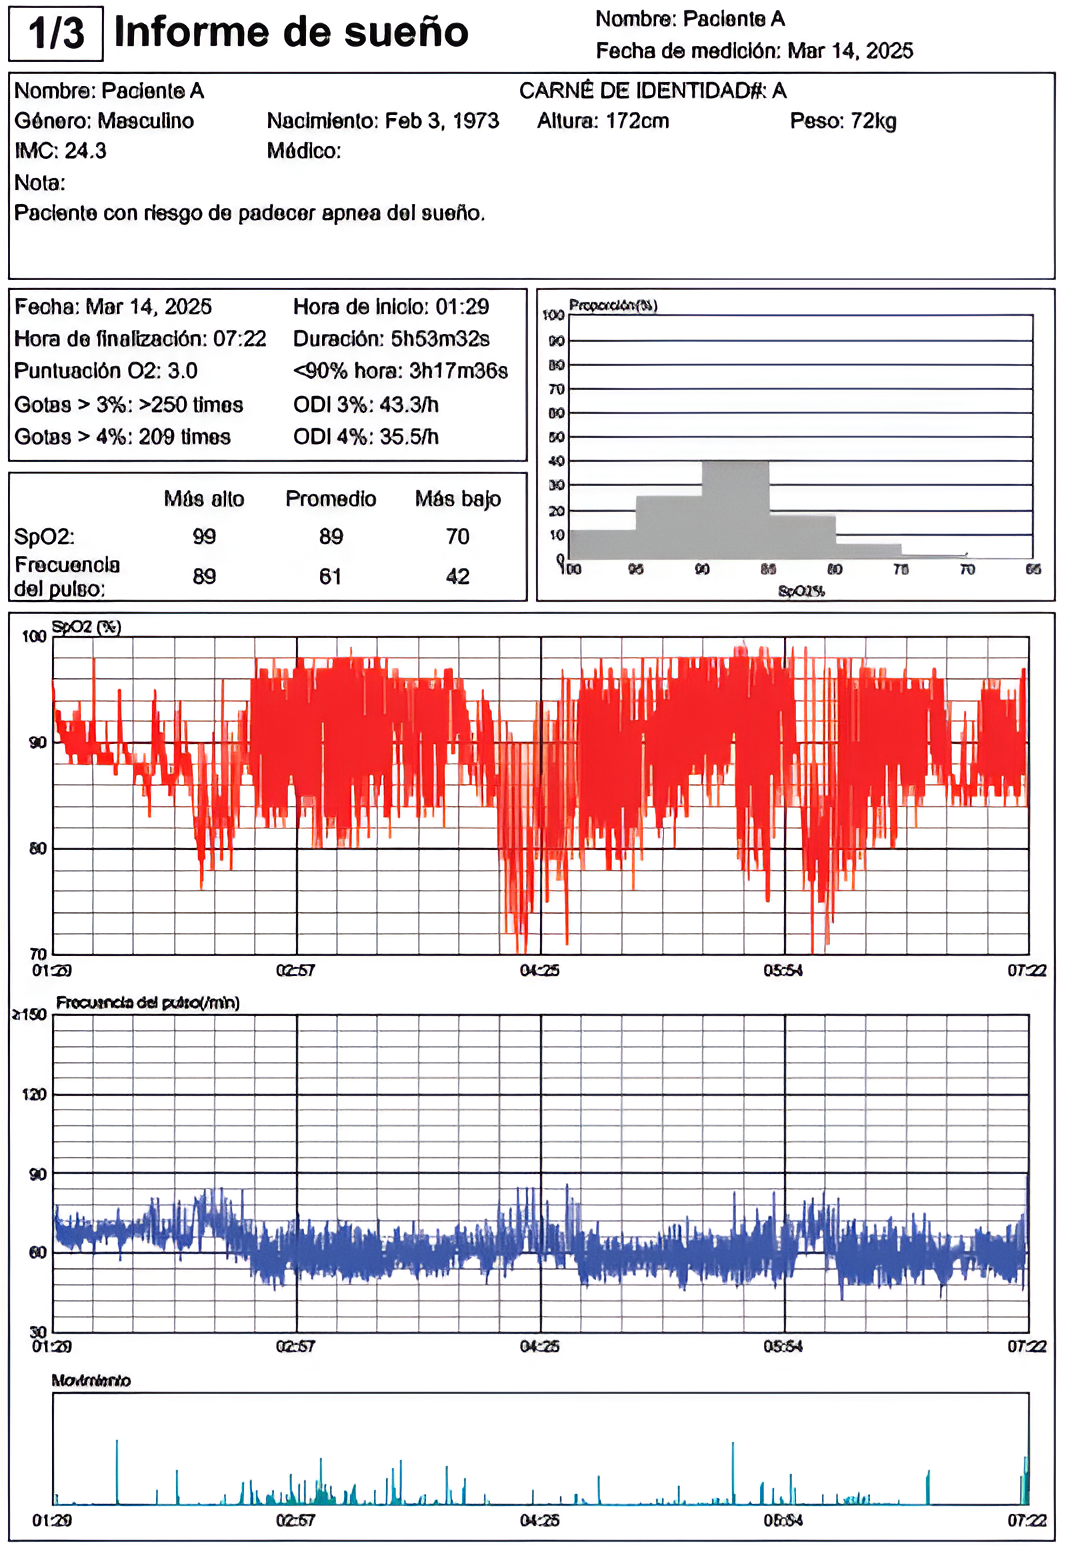
\includegraphics[width=1\textwidth]{img/informe_o2ring_pacienteA.png}
    \caption{Primera página del informe del dispositivo O2Ring para el Paciente A.}
    \label{fig:informe_o2ring}
\end{figure}


\section{Conclusión del estudio experimental}

Este anexo ha recogido todo el proceso experimental llevado a cabo para el desarrollo del sistema predictivo. A lo largo del trabajo se ha evaluado un conjunto diverso de algoritmos de clasificación, explorado técnicas de calibración e interpretabilidad, y finalmente desplegado un modelo funcional dentro de una aplicación web.

La validación externa con datos reales reveló fallos importantes, como la incapacidad del sistema para discriminar adecuadamente entre insomnio leve y apnea del sueño. Sin embargo, estos errores no invalidan el enfoque, sino que ponen de manifiesto la necesidad de enriquecer el entrenamiento con datos fisiológicos reales.

En conjunto, el estudio experimental demuestra que es viable desarrollar un sistema de predicción del tipo de trastorno del sueño basado en datos clínicos estructurados. No obstante, también subraya que la fiabilidad clínica de este tipo de sistemas depende en gran medida del tipo de variables disponibles y de su validación en entornos reales.

Este estudio no solo permitió desarrollar un sistema funcional, sino también comprender con mayor profundidad las limitaciones reales de los modelos clínicos basados únicamente en datos autodeclarados. El proceso completo ha sido esencial para identificar futuras líneas de mejora y consolidar una base sólida para trabajos posteriores.
